\chapter{Релейный регулятор}
{\bfseries Анонс:}\\\\
Работа с датчиком расстояния. Движение вдоль стенки. Релейный регулятор.\\\\
{\bfseries Цели:}
\begin{itemize}
	\item{}{\bfseries Обучающие:} Закрепить основы работы с сенсорами. Придумать и реализовать простейший способ автоматического управления.
	\item{}{\bfseries Развивающая:} Сформировать умения прослеживать причинно-следственные связи, анализировать информацию, применять полученные знания в новых ситуациях.\\
\end{itemize}	
{\bfseries Ход занятия:}\\\\
\begin{tabular}[h!]{lll}
	{\hyperlink{lesson15x1}{1. Организационный момент}}&{Презентация}&{(5 мин)}\\
	{\hyperlink{lesson15x2}{2. Остановка перед препятствием}}&{Практика + Рефлексия}&{(30 мин)}\\
	{\hyperlink{lesson15x3}{3. Движение вдоль стенки}}&{Практика}&{(60 мин)}\\
	{\hyperlink{lesson15x4}{4. Релейный регулятор}}&{Рефлексия}&{(20 мин)}\\
\end{tabular}\\\\

{\hypertarget{lesson15x1}{\blackBlueText{I. Организационный момент}}}\\\\	

Все задания могут выполняться в командах по 2 человека. Обсуждение вопросов второго блока происходит всем классом, затем по парам дети реализовывают предложенную программу и исправляют ее (п.6--7). В третьем блоке учащимся предлагается задача для самостоятельного решения и достаточное количество времени для творчества. По возможности следует не рассказывать решение, а задавать проблемные вопросы и подталкивать к самостоятельному поиску. В четвертом блоке совместно с учащимися происходит анализ основных моментов задачи и структуризация полученных знаний.\\\\

{\hypertarget{lesson15x2}{\blackBlueText{II. Остановка перед препятствием}}}\\\\

Раздайте учащимся следующий код:

\begin{figure}[h!]
	\begin{center}
		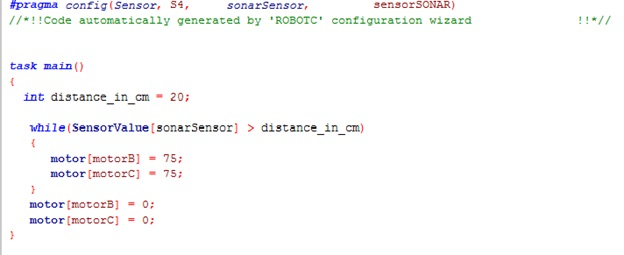
\includegraphics[width=1\linewidth]{chapters/chapter15/images/1}
		\caption{}
		\label{ris:image15x1}
	\end{center}
\end{figure}	

\newcounter{questionsStopSonar}
\begin{itemize}
	\renewcommand{\labelitemi}{\stepcounter{questionsStopSonar}\thequestionsStopSonar)}
	\item Как будет действовать робот с такой программой?
	\item На каком расстоянии должен остановиться робот от помехи? 
	\item  На каком расстоянии робот на самом деле остановиться от помехи?
	\item Любой ли робот будет останавливаться перед помехой на каком-то расстоянии при исполнении такой программы?
	\item  Какова должна быть конструкция робота, для выполнения задачи остановки?
	\item Сконструируйте такого робота и запустите на нем предложенную программу. На каком расстоянии от преграды остановился робот?
	\item Как надо модифицировать программу, что бы робот останавливался ровно на заданном расстоянии от преграды?
\end{itemize}
\clearpage
{\hypertarget{lesson15x3}{\blackBlueText{III. Движение вдоль стенки}}}\\\\	

Для выполнения следующего задания нам понадобиться знание еще одной новой команды: условия if (если).\\\\
if (условие)\\
\{\\
\indent Команда 1;\\
\indent Команда 2;\\
\}\\
else\\
\{\\
\indent Команда 3;\\
\indent Команда 4;\\
\}\\\\

Команды 1 и 2 будут выполнены, если условие в скобках было истинно, команды 3 и 4 , если ложно. Важно отметить, что в отличии от while, это не цикл! Т.е. условие проверяется один раз и после выполнения соответствующих команд программа начинает исполняться дальше.

Вопрос: Как заставить робота бесконечно проверять какое-то условие и действовать в соответствии с ним?\\\\

Задача: Проехать  вдоль стенки на расстоянии 20 см от нее. Стенка может иметь изгибы с углом не более 150 градусов.\\\\

{\hypertarget{lesson15x4}{\blackBlueText{IV. Релейный регулятор}}}\\\\

Любую робототехническую задачу можно разделить на две составляющие: конструкционную и программную. 

В конструкционной части задачи движения вдоль стенки было необходимо придумать движущуюся конструкцию и укрепить на этой основе датчик расстояния. В качестве основы можно было взять стандартную трехколесную тележку, скорость проезда роли не играла, так что необходимости в передаче или других конструкционных улучшениях здесь не было. Гораздо интереснее вопрос расположения датчика.

Представим изначально, что датчик измерения расстояния закреплен на оси ведущих колес, перпендикулярно направлению движения (pис.~\ref{ris:image15x2}). В таком случае при повороте тележки направо расстояние, измеряемое датчиком, увеличится, при повороте налево, тоже увеличится. Получается, управлять тележкой (поддерживать движение на постоянном расстоянии от стенки) с таким положением датчика не получится, по показаниям датчика мы не можем сказать приближается тележка к стене или удаляется.

\begin{figure}[h!]
	\begin{minipage}[h!]{0.5\linewidth}
		\begin{center}
			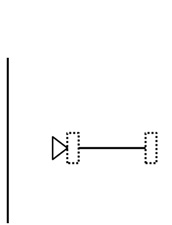
\includegraphics[width=0.8\linewidth]{chapters/chapter15/images/2}
			\caption{}
			\label{ris:image15x2}
		\end{center}
	\end{minipage}
	\begin{minipage}[h!]{0.5\linewidth}
		\begin{center}
			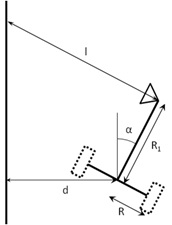
\includegraphics[width=0.8\linewidth]{chapters/chapter15/images/3}
			\caption{}
			\label{ris:image15x3}
		\end{center}
	\end{minipage}
\end{figure}

Выход из такой ситуации~--- расположить датчик на некотором расстоянии от оси ведущих колес (рис.~\ref{ris:image15x3}). В такой геометрии системы при повороте на небольшой угол направо расстояние, измеряемое датчиком, увеличивается, при повороте налево~--- уменьшается. Следует заметить, что при повороте налево на большой угол, показания датчика снова начнут увеличиваться. Можно показать, что чем дальше от ведущих колес мы расположим датчик расстояния, тем на больший угол сможем позволить поворачиваться тележку. 

{\slshape В группах 10--11классников, знакомых с понятиями синус и производная можно доказать это утверждение. Пусть расстояние между датчиком и осью ведущих колес \(R_1\). Пусть центр оси ведущих колес находится на расстоянии \(d\) от стенки, длина полуоси R, тележка повернута относительно стенки на угол \(\alpha\), при этом датчик расстояния измеряет расстояние \(l\).
	
	Расстояние, измеряемое датчиком можно выразить:
	
	\begin{equation}
	l=\frac{d+R_1sin\alpha}{cos\alpha}
	\end{equation}	
	
	Функция \(l(\alpha)\) имеет минимум, проходя через который показания датчика как раз таки и начнут снова увеличиваться. Граничный угол можно найти (приравняв производную \(l(\alpha)\) к нулю):
	
	\begin{equation}
	sin\alpha_{\mbox{\slshape гр}}=-\frac{R_1}{d}
	\label{formul15x4}
	\end{equation}	
	
	Равенство \ref{formul15x4} позволяет найти максимально допустимый угол поворота для тележки. При повороте на больший угол устойчивость системы легко может быть нарушена. Видно, что граничный угол действительно тем больше, чем больше расстояние \(R_1\).}

Программа движения робота должна при любом отклонении его от воображаемой линии в 20 см от стенки возвращать его обратно. Т.е. если стенка находится слева, как на рис., когда показания датчика становятся больше 20 см, тележку следует начать поворачивать налево, когда меньше – поворачивать направо. Радиусы поворота не важны, так что достаточна на один мотор просто подавать большую мощность, чем на другой. Возможная программа выглядит так:

\begin{figure}[h!]
	\begin{center}
		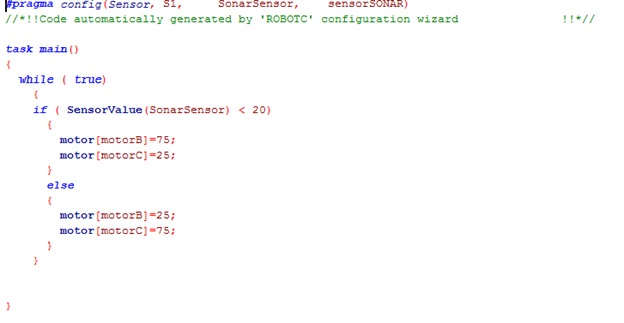
\includegraphics[width=1\linewidth]{chapters/chapter15/images/4}
		\caption{}
		\label{ris:image15x4}
	\end{center}
\end{figure}

Стоит отметить, что дети, даже поняв идею программы, обязательно включают в перечень случаев SensorValue(SonarSensor)=20 и указание ехать прямо (равные напряжение на моторы)  в этом случае. Представляется важным обратить на это внимание и пояснить, что в любой реальной ситуации робот не поедет ровно в 20 см от стенки, что-то обязательно выведет его из положения равновесия и его траектория будет всегда представлять собой волнистую линию, в среднем располагающуюся в 20 см.

Выше написанный алгоритм носит название релейного регулятора. Релейный регулятор~--- тип обратной связи, при котором регистрируется только 2 типа сигнала от датчика~--- «есть~--- нет», а точнее «больше некоторого порога~--- меньше некоторого порога». При этом на управляемый элемент также подается 2 типа сигнала. Логику релейного регулятора можно проиллюстрировать следующим примером: Если датчик касания нажат~--- крутить мотор с мощностью 70 \%, если датчик касания не нажат~--- крутить мотор с мощностью 30 \%. Как видно, 2 типа сигнала от датчика и 2 типа управляющего сигнала на мотор. С точки зрения программирования релейный регулятор чаще всего описывается следующей блок схемой:

\begin{figure}[h!]
	\begin{center}
		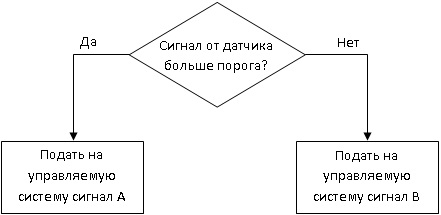
\includegraphics[width=1\linewidth]{chapters/chapter15/images/5}
		\caption{}
		\label{ris:image15x5}
	\end{center}
\end{figure}